
%% bare_conf.tex
%% V1.4b
%% 2015/08/26
%% by Michael Shell
%% See:
%% http://www.michaelshell.org/
%% for current contact information.
%%
%% This is a skeleton file demonstrating the use of IEEEtran.cls
%% (requires IEEEtran.cls version 1.8b or later) with an IEEE
%% conference paper.
%%
%% Support sites:
%% http://www.michaelshell.org/tex/ieeetran/
%% http://www.ctan.org/pkg/ieeetran
%% and
%% http://www.ieee.org/

%%*************************************************************************
%% Legal Notice:
%% This code is offered as-is without any warranty either expressed or
%% implied; without even the implied warranty of MERCHANTABILITY or
%% FITNESS FOR A PARTICULAR PURPOSE! 
%% User assumes all risk.
%% In no event shall the IEEE or any contributor to this code be liable for
%% any damages or losses, including, but not limited to, incidental,
%% consequential, or any other damages, resulting from the use or misuse
%% of any information contained here.
%%
%% All comments are the opinions of their respective authors and are not
%% necessarily endorsed by the IEEE.
%%
%% This work is distributed under the LaTeX Project Public License (LPPL)
%% ( http://www.latex-project.org/ ) version 1.3, and may be freely used,
%% distributed and modified. A copy of the LPPL, version 1.3, is included
%% in the base LaTeX documentation of all distributions of LaTeX released
%% 2003/12/01 or later.
%% Retain all contribution notices and credits.
%% ** Modified files should be clearly indicated as such, including  **
%% ** renaming them and changing author support contact information. **
%%*************************************************************************


% *** Authors should verify (and, if needed, correct) their LaTeX system  ***
% *** with the testflow diagnostic prior to trusting their LaTeX platform ***
% *** with production work. The IEEE's font choices and paper sizes can   ***
% *** trigger bugs that do not appear when using other class files.       ***                          ***
% The testflow support page is at:
% http://www.michaelshell.org/tex/testflow/



\documentclass[conference]{IEEEtran}
% Some Computer Society conferences also require the compsoc mode option,
% but others use the standard conference format.
%
% If IEEEtran.cls has not been installed into the LaTeX system files,
% manually specify the path to it like:
% \documentclass[conference]{../sty/IEEEtran}





% Some very useful LaTeX packages include:
% (uncomment the ones you want to load)


% *** MISC UTILITY PACKAGES ***
%
%\usepackage{ifpdf}
% Heiko Oberdiek's ifpdf.sty is very useful if you need conditional
% compilation based on whether the output is pdf or dvi.
% usage:
% \ifpdf
%   % pdf code
% \else
%   % dvi code
% \fi
% The latest version of ifpdf.sty can be obtained from:
% http://www.ctan.org/pkg/ifpdf
% Also, note that IEEEtran.cls V1.7 and later provides a builtin
% \ifCLASSINFOpdf conditional that works the same way.
% When switching from latex to pdflatex and vice-versa, the compiler may
% have to be run twice to clear warning/error messages.






% *** CITATION PACKAGES ***
%
%\usepackage{cite}
% cite.sty was written by Donald Arseneau
% V1.6 and later of IEEEtran pre-defines the format of the cite.sty package
% \cite{} output to follow that of the IEEE. Loading the cite package will
% result in citation numbers being automatically sorted and properly
% "compressed/ranged". e.g., [1], [9], [2], [7], [5], [6] without using
% cite.sty will become [1], [2], [5]--[7], [9] using cite.sty. cite.sty's
% \cite will automatically add leading space, if needed. Use cite.sty's
% noadjust option (cite.sty V3.8 and later) if you want to turn this off
% such as if a citation ever needs to be enclosed in parenthesis.
% cite.sty is already installed on most LaTeX systems. Be sure and use
% version 5.0 (2009-03-20) and later if using hyperref.sty.
% The latest version can be obtained at:
% http://www.ctan.org/pkg/cite
% The documentation is contained in the cite.sty file itself.






% *** GRAPHICS RELATED PACKAGES ***
%
\ifCLASSINFOpdf
  % \usepackage[pdftex]{graphicx}
  % declare the path(s) where your graphic files are
  % \graphicspath{{../pdf/}{../jpeg/}}
  % and their extensions so you won't have to specify these with
  % every instance of \includegraphics
  % \DeclareGraphicsExtensions{.pdf,.jpeg,.png}
\else
  % or other class option (dvipsone, dvipdf, if not using dvips). graphicx
  % will default to the driver specified in the system graphics.cfg if no
  % driver is specified.
  % \usepackage[dvips]{graphicx}
  % declare the path(s) where your graphic files are
  % \graphicspath{{../eps/}}
  % and their extensions so you won't have to specify these with
  % every instance of \includegraphics
  % \DeclareGraphicsExtensions{.eps}
\fi
% graphicx was written by David Carlisle and Sebastian Rahtz. It is
% required if you want graphics, photos, etc. graphicx.sty is already
% installed on most LaTeX systems. The latest version and documentation
% can be obtained at: 
% http://www.ctan.org/pkg/graphicx
% Another good source of documentation is "Using Imported Graphics in
% LaTeX2e" by Keith Reckdahl which can be found at:
% http://www.ctan.org/pkg/epslatex
%
% latex, and pdflatex in dvi mode, support graphics in encapsulated
% postscript (.eps) format. pdflatex in pdf mode supports graphics
% in .pdf, .jpeg, .png and .mps (metapost) formats. Users should ensure
% that all non-photo figures use a vector format (.eps, .pdf, .mps) and
% not a bitmapped formats (.jpeg, .png). The IEEE frowns on bitmapped formats
% which can result in "jaggedy"/blurry rendering of lines and letters as
% well as large increases in file sizes.
%
% You can find documentation about the pdfTeX application at:
% http://www.tug.org/applications/pdftex





% *** MATH PACKAGES ***
%
%\usepackage{amsmath}
% A popular package from the American Mathematical Society that provides
% many useful and powerful commands for dealing with mathematics.
%
% Note that the amsmath package sets \interdisplaylinepenalty to 10000
% thus preventing page breaks from occurring within multiline equations. Use:
%\interdisplaylinepenalty=2500
% after loading amsmath to restore such page breaks as IEEEtran.cls normally
% does. amsmath.sty is already installed on most LaTeX systems. The latest
% version and documentation can be obtained at:
% http://www.ctan.org/pkg/amsmath





% *** SPECIALIZED LIST PACKAGES ***
%
%\usepackage{algorithmic}
% algorithmic.sty was written by Peter Williams and Rogerio Brito.
% This package provides an algorithmic environment fo describing algorithms.
% You can use the algorithmic environment in-text or within a figure
% environment to provide for a floating algorithm. Do NOT use the algorithm
% floating environment provided by algorithm.sty (by the same authors) or
% algorithm2e.sty (by Christophe Fiorio) as the IEEE does not use dedicated
% algorithm float types and packages that provide these will not provide
% correct IEEE style captions. The latest version and documentation of
% algorithmic.sty can be obtained at:
% http://www.ctan.org/pkg/algorithms
% Also of interest may be the (relatively newer and more customizable)
% algorithmicx.sty package by Szasz Janos:
% http://www.ctan.org/pkg/algorithmicx




% *** ALIGNMENT PACKAGES ***
%
%\usepackage{array}
% Frank Mittelbach's and David Carlisle's array.sty patches and improves
% the standard LaTeX2e array and tabular environments to provide better
% appearance and additional user controls. As the default LaTeX2e table
% generation code is lacking to the point of almost being broken with
% respect to the quality of the end results, all users are strongly
% advised to use an enhanced (at the very least that provided by array.sty)
% set of table tools. array.sty is already installed on most systems. The
% latest version and documentation can be obtained at:
% http://www.ctan.org/pkg/array


% IEEEtran contains the IEEEeqnarray family of commands that can be used to
% generate multiline equations as well as matrices, tables, etc., of high
% quality.




% *** SUBFIGURE PACKAGES ***
%\ifCLASSOPTIONcompsoc
%  \usepackage[caption=false,font=normalsize,labelfont=sf,textfont=sf]{subfig}
%\else
%  \usepackage[caption=false,font=footnotesize]{subfig}
%\fi
% subfig.sty, written by Steven Douglas Cochran, is the modern replacement
% for subfigure.sty, the latter of which is no longer maintained and is
% incompatible with some LaTeX packages including fixltx2e. However,
% subfig.sty requires and automatically loads Axel Sommerfeldt's caption.sty
% which will override IEEEtran.cls' handling of captions and this will result
% in non-IEEE style figure/table captions. To prevent this problem, be sure
% and invoke subfig.sty's "caption=false" package option (available since
% subfig.sty version 1.3, 2005/06/28) as this is will preserve IEEEtran.cls
% handling of captions.
% Note that the Computer Society format requires a larger sans serif font
% than the serif footnote size font used in traditional IEEE formatting
% and thus the need to invoke different subfig.sty package options depending
% on whether compsoc mode has been enabled.
%
% The latest version and documentation of subfig.sty can be obtained at:
% http://www.ctan.org/pkg/subfig




% *** FLOAT PACKAGES ***
%
%\usepackage{fixltx2e}
% fixltx2e, the successor to the earlier fix2col.sty, was written by
% Frank Mittelbach and David Carlisle. This package corrects a few problems
% in the LaTeX2e kernel, the most notable of which is that in current
% LaTeX2e releases, the ordering of single and double column floats is not
% guaranteed to be preserved. Thus, an unpatched LaTeX2e can allow a
% single column figure to be placed prior to an earlier double column
% figure.
% Be aware that LaTeX2e kernels dated 2015 and later have fixltx2e.sty's
% corrections already built into the system in which case a warning will
% be issued if an attempt is made to load fixltx2e.sty as it is no longer
% needed.
% The latest version and documentation can be found at:
% http://www.ctan.org/pkg/fixltx2e


%\usepackage{stfloats}
% stfloats.sty was written by Sigitas Tolusis. This package gives LaTeX2e
% the ability to do double column floats at the bottom of the page as well
% as the top. (e.g., "\begin{figure*}[!b]" is not normally possible in
% LaTeX2e). It also provides a command:
%\fnbelowfloat
% to enable the placement of footnotes below bottom floats (the standard
% LaTeX2e kernel puts them above bottom floats). This is an invasive package
% which rewrites many portions of the LaTeX2e float routines. It may not work
% with other packages that modify the LaTeX2e float routines. The latest
% version and documentation can be obtained at:
% http://www.ctan.org/pkg/stfloats
% Do not use the stfloats baselinefloat ability as the IEEE does not allow
% \baselineskip to stretch. Authors submitting work to the IEEE should note
% that the IEEE rarely uses double column equations and that authors should try
% to avoid such use. Do not be tempted to use the cuted.sty or midfloat.sty
% packages (also by Sigitas Tolusis) as the IEEE does not format its papers in
% such ways.
% Do not attempt to use stfloats with fixltx2e as they are incompatible.
% Instead, use Morten Hogholm'a dblfloatfix which combines the features
% of both fixltx2e and stfloats:
%
% \usepackage{dblfloatfix}
% The latest version can be found at:
% http://www.ctan.org/pkg/dblfloatfix




% *** PDF, URL AND HYPERLINK PACKAGES ***
%
%\usepackage{url}
% url.sty was written by Donald Arseneau. It provides better support for
% handling and breaking URLs. url.sty is already installed on most LaTeX
% systems. The latest version and documentation can be obtained at:
% http://www.ctan.org/pkg/url
% Basically, \url{my_url_here}.




% *** Do not adjust lengths that control margins, column widths, etc. ***
% *** Do not use packages that alter fonts (such as pslatex).         ***
% There should be no need to do such things with IEEEtran.cls V1.6 and later.
% (Unless specifically asked to do so by the journal or conference you plan
% to submit to, of course. )


% correct bad hyphenation here
\hyphenation{op-tical net-works semi-conduc-tor}

\usepackage[portuges]{babel}
\usepackage[utf8]{inputenc}
\usepackage{cite}
\usepackage{graphicx,url}

\begin{document}
%
% paper title
% Titles are generally capitalized except for words such as a, an, and, as,
% at, but, by, for, in, nor, of, on, or, the, to and up, which are usually
% not capitalized unless they are the first or last word of the title.
% Linebreaks \\ can be used within to get better formatting as desired.
% Do not put math or special symbols in the title.
\title{Qualidade de Serviço em serviços de nuvem: uma análise do OpenStack}


% author names and affiliations
% use a multiple column layout for up to three different
% affiliations
\author{\IEEEauthorblockN{Emilie Trindade de Morais}
\IEEEauthorblockA{Faculdade do Gama, Universidade de Brasília
  (UnB)\\
  Gama, DF -- Brasil\\
Email: emiliemoraist@gmail.com}
\and
\IEEEauthorblockN{Ítalo Paiva Batista}
\IEEEauthorblockA{Faculdade do Gama, Universidade de Brasília
  (UnB)\\
  Gama, DF -- Brasil\\
Email: italopaivab@gmail.com}
}
% conference papers do not typically use \thanks and this command
% is locked out in conference mode. If really needed, such as for
% the acknowledgment of grants, issue a \IEEEoverridecommandlockouts
% after \documentclass

% for over three affiliations, or if they all won't fit within the width
% of the page, use this alternative format:
% 
%\author{\IEEEauthorblockN{Michael Shell\IEEEauthorrefmark{1},
%Homer Simpson\IEEEauthorrefmark{2},
%James Kirk\IEEEauthorrefmark{3}, 
%Montgomery Scott\IEEEauthorrefmark{3} and
%Eldon Tyrell\IEEEauthorrefmark{4}}
%\IEEEauthorblockA{\IEEEauthorrefmark{1}School of Electrical and Computer Engineering\\
%Georgia Institute of Technology,
%Atlanta, Georgia 30332--0250\\ Email: see http://www.michaelshell.org/contact.html}
%\IEEEauthorblockA{\IEEEauthorrefmark{2}Twentieth Century Fox, Springfield, USA\\
%Email: homer@thesimpsons.com}
%\IEEEauthorblockA{\IEEEauthorrefmark{3}Starfleet Academy, San Francisco, California 96678-2391\\
%Telephone: (800) 555--1212, Fax: (888) 555--1212}
%\IEEEauthorblockA{\IEEEauthorrefmark{4}Tyrell Inc., 123 Replicant Street, Los Angeles, California 90210--4321}}




% use for special paper notices
%\IEEEspecialpapernotice{(Invited Paper)}




% make the title area
\maketitle

% As a general rule, do not put math, special symbols or citations
% in the abstract
\begin{abstract}
The abstract goes here.
\end{abstract}

% no keywords




% For peer review papers, you can put extra information on the cover
% page as needed:
% \ifCLASSOPTIONpeerreview
% \begin{center} \bfseries EDICS Category: 3-BBND \end{center}
% \fi
%
% For peerreview papers, this IEEEtran command inserts a page break and
% creates the second title. It will be ignored for other modes.
\IEEEpeerreviewmaketitle



\section{Introdução}
% no \IEEEPARstart
Portanto, o objetivo deste trabalho é identificar as métricas de QoS que a ferramenta OpenStack fornece aos seus usuários. % MELHORAR

\section{Serviços de nuvem}
De acordo com \citeonline{armbrust2010view}, a computação em nuvem refere-se a aplicações que entregam serviços a partir da internet. 
Os quais são providos através de hardware e software presentes em \textit{data centers}. São serviços que oferecem mecanismos
para prover acesso aos usuários virtualmente a recursos ilimitados baseado no modelo \textit{payper-use}, ou seja, pagamento
pelo uso. \cite{sefraoui2012openstack}

Com a finalidade de prover esses serviços a computação em nuvem é estruturada em três módulos: Infraestrutura como serviço(IaaS),
Plataforma como serviço(PaaS) e Software como serviço (SaaS), as quais estão ordenadas por nível de abstração, do mais baixo 
para o mais alto, respectivamente \cite{rehman2011teaching, sefraoui2012openstack, armbrust2010view, mell2011nist}. 
Essa estrutura pode ser vista na Figura \ref{fig:cloud_structure}.

\begin{figure}[ht]
\centering
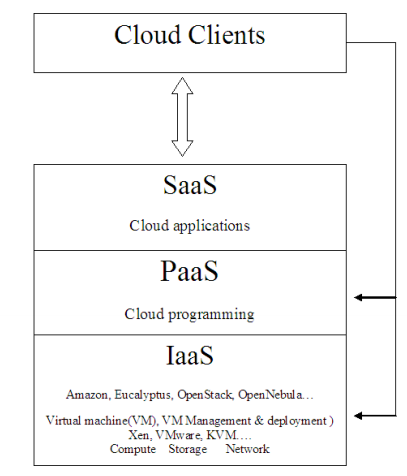
\includegraphics[width=.3\textwidth]{figuras/cloud_structure.png}
\caption{Estrutura de serviços da computação em nuvem. Fonte: \cite{sefraoui2012openstack}}
\label{fig:cloud_structure}
\end{figure}

\citeonline{sefraoui2012openstack}, afirma que a IaaS é onde o recurso de hardware é provido em forma de máquinas vituais. O cliente mantém
as aplicações, bancos de dados e servidores enquanto o servidor mantém a virtualização da nuvem, o hardware, o armazenamento e as redes.
Para \citeonline{bhardwaj2010cloud}, é o serviço de entrega de hardware (servidor, armazenamento e rede) e software associado 
(sistema de arquivos e virtualização de sistemas).

De acordo com \citeonline{leite2016influencia} (apud \cite{mell2011nist}), os serviços de nuvens devem possuir as seguintes
características: autoatendimento sob demanda, amplo acesso a rede,
agrupamento de recursos, elasticidade rápida e medição de serviço.

\subsection{Qualidade de Serviço em nuvem}

A medição dos serviços de nuvem é uma das características essenciais de acordo com 
\citeonline{mell2011nist}. \citeonline{leite2016influencia} afirma que essas medições proporcionam
transparência ao provedor e ao cliente. Medir os serviços de nuvem auxiliam no 
cumprimento dos níveis de serviços acordados.


\citeonline{leite2016influencia} trata a qualidade de serviço em duas abordagens:
uma relacionada à rede e outra em nível de aplicação. Em relação a rede são tratados
os requisitos para garantir a qualidade do serviço. Em nível de aplicação são tratados
os atributos que implicam no cumprimento dos níveis de serviço acordado. 
Neste trabalho será tratada a qualidade de serviço do ponto de vista da aplicação.

\citeonline{siegel2012cloud} apresentam métricas para cálculo dos benefícios e riscos
de serviços de computação em nuvem. Características como prestação de contas, agilidade,
garantia, financeira, desempenho, segurança e privacidade e usabilidade. 

%Características como memória, processamento, enlace e sistemas operacionais suportados
%são comumente relacionadas com a qualidade dos serviços prestados. Assim como a 
%disponibilidade, segurança, privacidade e integridade. \cite{leite2016influencia}


% Métricas: 
  % Principais: memória, processamento, enlace e SO
  % Outras: Disponibilidade, Segurança, Privacidade, Integridade



\subsection{Infraestrutura como serviço}

\citeonline{bhardwaj2010cloud} estabelece os seguintes serviços a serem providos 
por IaaS: Infraestrutura virtual (servidor, armazenamento e rede);
Implantação de aplicativos baseados na Web para fácil disponibilização sob demanda; Balanceamento de carga; 
Estabelecimento de acordos de nível de serviço com os clientes;  Segurança dos CPUs, dados e rede;
e Gestão e provisionamento de conta.

\subsection{OpenStack}

O OpenStack é uma plataforma de computação em nuvem de código aberto que permite o gerenciamento e desenvolvimento 
de uma infraestrutura de computação em nuvem em um \textit{datacenter}, que é mantido pela 
\textit{OpenStack Foundation} \cite{openstack} \cite{bui2016}.

O OpenStack fornece serviços de computação em nuvem no modelo IaaS e consiste em um grupo de subprojetos (cada subprojeto é um módulo 
do OpenStack) inter-relacionados 
que controlam um conjunto de recursos de processamento (subprojeto \textit{Nova}), armazenamento (subprojetos \textit{Cinder} e \textit{Swift}),
e de rede (subprojeto \textit{Neutron}) em uma infraestrutura de computação em nuvem \cite{openstack} \cite{bui2016}.
Além desses subprojetos apresentados, o OpenStack conta com alguns serviços compartilhados entre os diferentes módulos, como o serviço de 
autenticação e autorização (subprojeto \textit{Keystone}), serviço de gerenciamento de imagens (subprojeto \textit{Glance}) e o serviço de 
telemetria (subprojeto \textit{Ceilometer}) \cite{openstack}.

O gerenciamento e controle da infraestrutura da nuvem pelo OpenStack pode ser realizado por meio de uma aplicação \textit{web}
(subprojeto \textit{Horizon}), APIs para linha de comando e/ou APIs RESTful \cite{bui2016} \cite{openstack}.

A Figura \ref{fig:openstack_architecture} ilustra a arquitetura conceitual do OpenStack, apresentando o relacionamento entre os
módulos que o compõe.

\begin{figure*}[ht]
\centering
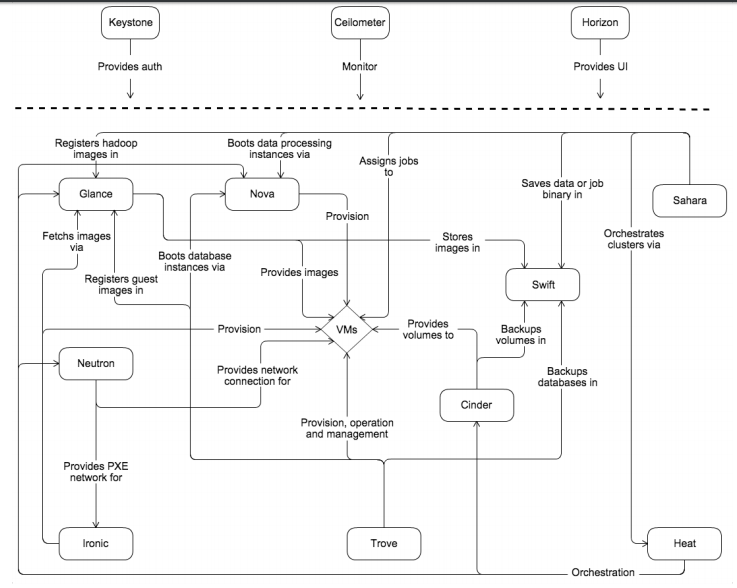
\includegraphics[width=.8\textwidth]{figuras/openstack_architecture.png}
\caption{Arquitetura conceitual do OpenStack. Fonte: \cite{openstack}}
\label{fig:openstack_architecture}
\end{figure*}

\section{Metodologia}

Para atingir o objetivo deste trabalho foi utilizada a metodologia apresentada na Figura \ref{metodologia},
cujas etapas são explicadas a seguir.


\begin{figure}[ht]
  \centering
  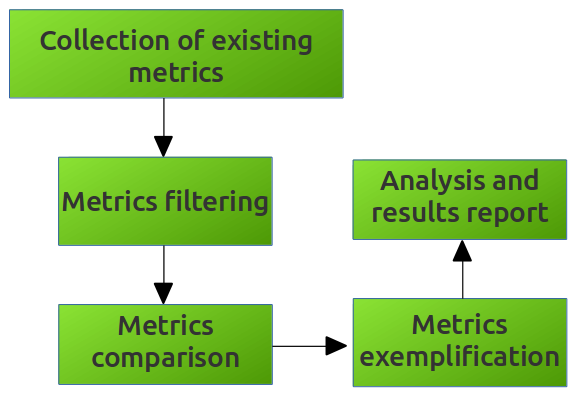
\includegraphics[width=.3\textwidth]{figuras/metodologia.png}
  \caption{Metodologia proposta. Fonte: Autor.}
  \label{metodologia}
\end{figure}


\begin{itemize}
 \item \textbf{Levantamento das métricas existentes} - Esta etapa consistiu em consultar na literatura as métricas de QoS para
	serviços de nuvem e documentá-las;
 \item \textbf{Filtragem das métricas} - A partir das métricas levantadas com a revisão da literatura, a próxima etapa consistiu em 
	identificar quais métricas se aplicam para o modelo de serviço IaaS, pois pode acontecer de algumas métricas se encaixarem
	mais aos outros modelos de serviço e não serem propícias ao modelo IaaS, devido às suas características peculiares. Além disso,
	métricas muito complexas (que exigem muitos insumos, insumos complicados de se obter e/ou cálculos mais complexos) foram descartadas,
	a fim de obter métricas mais passíveis da ferramenta fornecer;
 \item \textbf{Levantamento das métricas do OpenStack} - Esta etapa consistiu em verificar quais métricas a ferramenta oferecia,
	realizando uma simples coleta das métricas presentes no OpenStack a partir da execução da ferramenta em um cenário de teste 
	e análise da documentação.
	Esta etapa englobou as seguintes atividades:
	\subitem - \emph{\textbf{Caracterizar cenário/contexto}}: Nesta atividade descreveu-se o contexto da execução da ferramenta,
		 considerando itens como ambiente para execução do teste, versão da ferramenta utilizada, topologia utilizada, ferramentas
		 e recursos disponíveis;
	\subitem - \emph{\textbf{Elaborar plano de medição}}: Nesta atividade um plano de medição resumido foi criado para guiar a medição
		 a ser feita;
	\subitem - \emph{\textbf{Coletar dados}}: Nesta atividade as métricas foram coletadas e documentadas, seguindo o
		 plano de medição definido anteriormente.
 \item \textbf{Confronto das métricas} - Esta etapa consistiu em comparar as métricas encontradas na literatura com as métricas
	identificadas no OpenStack, para verificar quais métricas propostas na literatura são percebidas na prática no OpenStack;
 \item \textbf{Análise e redação dos resultados}: Nesta etapa os resultados obtidos na etapa anterior foram interpretados e documentados.
\end{itemize}


\section{Conclusão}
The conclusion goes here.



% \subsection{Subsection Heading Here}
% Subsection text here.
% 
% 
% \subsubsection{Subsubsection Heading Here}
% Subsubsection text here.


% An example of a floating figure using the graphicx package.
% Note that \label must occur AFTER (or within) \caption.
% For figures, \caption should occur after the \includegraphics.
% Note that IEEEtran v1.7 and later has special internal code that
% is designed to preserve the operation of \label within \caption
% even when the captionsoff option is in effect. However, because
% of issues like this, it may be the safest practice to put all your
% \label just after \caption rather than within \caption{}.
%
% Reminder: the "draftcls" or "draftclsnofoot", not "draft", class
% option should be used if it is desired that the figures are to be
% displayed while in draft mode.
%
%\begin{figure}[!t]
%\centering
%\includegraphics[width=2.5in]{myfigure}
% where an .eps filename suffix will be assumed under latex, 
% and a .pdf suffix will be assumed for pdflatex; or what has been declared
% via \DeclareGraphicsExtensions.
%\caption{Simulation results for the network.}
%\label{fig_sim}
%\end{figure}

% Note that the IEEE typically puts floats only at the top, even when this
% results in a large percentage of a column being occupied by floats.


% An example of a double column floating figure using two subfigures.
% (The subfig.sty package must be loaded for this to work.)
% The subfigure \label commands are set within each subfloat command,
% and the \label for the overall figure must come after \caption.
% \hfil is used as a separator to get equal spacing.
% Watch out that the combined width of all the subfigures on a 
% line do not exceed the text width or a line break will occur.
%
% \begin{figure*}[!t]
% \centering
% \subfloat[Case I]{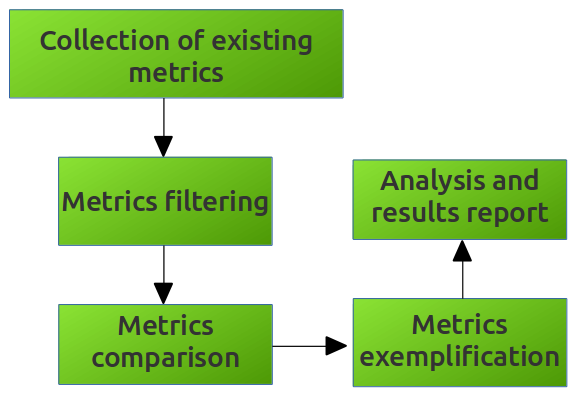
\includegraphics[width=2.5in]{figuras/metodologia}%
% \label{fig_first_case}}
% \hfil
% \subfloat[Case II]{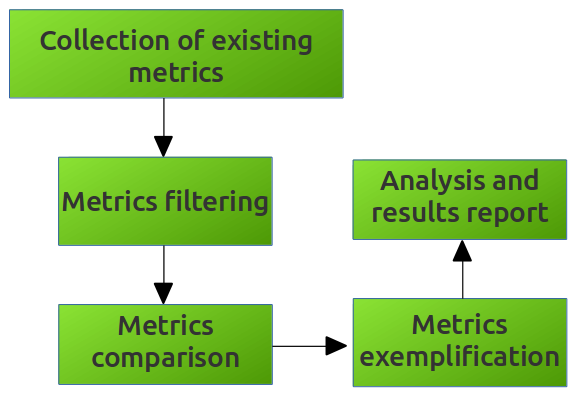
\includegraphics[width=2.5in]{figuras/metodologia}%
% \label{fig_second_case}}
% \caption{Simulation results for the network.}
% \label{fig_sim}
% \end{figure*}
%
% Note that often IEEE papers with subfigures do not employ subfigure
% captions (using the optional argument to \subfloat[]), but instead will
% reference/describe all of them (a), (b), etc., within the main caption.
% Be aware that for subfig.sty to generate the (a), (b), etc., subfigure
% labels, the optional argument to \subfloat must be present. If a
% subcaption is not desired, just leave its contents blank,
% e.g., \subfloat[].


% An example of a floating table. Note that, for IEEE style tables, the
% \caption command should come BEFORE the table and, given that table
% captions serve much like titles, are usually capitalized except for words
% such as a, an, and, as, at, but, by, for, in, nor, of, on, or, the, to
% and up, which are usually not capitalized unless they are the first or
% last word of the caption. Table text will default to \footnotesize as
% the IEEE normally uses this smaller font for tables.
% The \label must come after \caption as always.
%
%\begin{table}[!t]
%% increase table row spacing, adjust to taste
%\renewcommand{\arraystretch}{1.3}
% if using array.sty, it might be a good idea to tweak the value of
% \extrarowheight as needed to properly center the text within the cells
%\caption{An Example of a Table}
%\label{table_example}
%\centering
%% Some packages, such as MDW tools, offer better commands for making tables
%% than the plain LaTeX2e tabular which is used here.
%\begin{tabular}{|c||c|}
%\hline
%One & Two\\
%\hline
%Three & Four\\
%\hline
%\end{tabular}
%\end{table}


% Note that the IEEE does not put floats in the very first column
% - or typically anywhere on the first page for that matter. Also,
% in-text middle ("here") positioning is typically not used, but it
% is allowed and encouraged for Computer Society conferences (but
% not Computer Society journals). Most IEEE journals/conferences use
% top floats exclusively. 
% Note that, LaTeX2e, unlike IEEE journals/conferences, places
% footnotes above bottom floats. This can be corrected via the
% \fnbelowfloat command of the stfloats package.

% conference papers do not normally have an appendix


% use section* for acknowledgment
% \section*{Acknowledgment}


% The authors would like to thank...





% trigger a \newpage just before the given reference
% number - used to balance the columns on the last page
% adjust value as needed - may need to be readjusted if
% the document is modified later
%\IEEEtriggeratref{8}
% The "triggered" command can be changed if desired:
%\IEEEtriggercmd{\enlargethispage{-5in}}

% references section

% can use a bibliography generated by BibTeX as a .bbl file
% BibTeX documentation can be easily obtained at:
% http://mirror.ctan.org/biblio/bibtex/contrib/doc/
% The IEEEtran BibTeX style support page is at:
% http://www.michaelshell.org/tex/ieeetran/bibtex/
%\bibliographystyle{IEEEtran}
% argument is your BibTeX string definitions and bibliography database(s)
%\bibliography{IEEEabrv,../bib/paper}
%
% <OR> manually copy in the resultant .bbl file
% set second argument of \begin to the number of references
% (used to reserve space for the reference number labels box)

\bibliographystyle{IEEEtran}
\bibliography{IEEEabrv, references}
% \begin{thebibliography}{1}
% 
% \bibitem{IEEEhowto:kopka}
% H.~Kopka and P.~W. Daly, \emph{A Guide to \LaTeX}, 3rd~ed.\hskip 1em plus
%   0.5em minus 0.4em\relax Harlow, England: Addison-Wesley, 1999.
% 
% \end{thebibliography}




% that's all folks
\end{document}


